\documentclass[english,oneside,color]{htldipl}
% Zulässige Class Options: 
%   Hauptsprache: german (default), english
%   Doppelseitig: oneside (default), twoside
%   Syntax-Highlighting: color (default), black

% die folgende Zeile einkommentieren für Arial-Ähnliche Schriftart
%\renewcommand{\familydefault}{\sfdefault}

\graphicspath{{images/}}    % Bilderverzeichnis


\include{Settings}

\makeglossaries
\loadglsentries{glossary}					%beinhaltet Daten für das Glossar
\addbibresource{literatur.bib}     %beinhaltet Daten für das Literarturverzeichnis

%%%----------------------------------------------------------
\begin{document}
%%%----------------------------------------------------------
%Einstellungen an die eigene Diplomarbeit anpassen
\title{AWS DeepRacer}
\abteilung{Informatik}
%\schwerpunkt{} wenn kein Ausbildungsschwerpunkt vorhanden ist z.B. Informatik
\schwerpunkt{Ausbildungsschwerpunkt Machine Learning}
\studienort{Wiener Neustadt}
\schule{HTBLuVA Wiener Neustadt}
\schullogo{htl.jpeg}
\abgabejahr{2020/21}
\betreuerA{Dipl.-Ing. Harald Haberstroh}
\betreuerB{}
\betreuerC{}
\betreuerD{}
%\betreuerD{} leer lassen wenn nicht vorhanden
\schuelerA{Sebastian ROHRER}
\evidenzA{5BHIF-XX}
\subthemaA{--}
\schuelerB{Florian SCHWARZL}
\evidenzB{5BHIF-XX}
\subthemaB{--}
\schuelerC{test}
\evidenzC{}
\subthemaC{}
\schuelerD{}
\evidenzD{}
\subthemaD{}
\schuelerE{}
\evidenzE{}
\subthemaE{}
%\schuelerE{} leer lassen wenn nicht vorhanden
%\evidenzE{}
%\subthemaE{}



%%%----------------------------------------------------------
\frontmatter
\maketitle
\tableofcontents
%%%----------------------------------------------------------

\chapter{Vorwort}

%Übrigens, hier im Vorwort kann man kurz auf die Entstehung  des Dokuments eingehen.
%Hier ist auch der Platz für allfällige Danksagungen (\zB an den Betreuer, 
%den Begutachter, die Familie, den Hund, ...), Widmungen und philosophische 
%Anmerkungen. Das sollte man allerdings auch nicht übertreiben und sich auf 
%einen Umfang von maximal zwei Seiten beschränken.

This is \textbf{Version \htldiplDate} of our diploma thesis created in LaTex, based on the template provided by Wolfgang Schermann.
During the creation of this document we were able to take a glimpse at the endless possibilities of machine learning.


				%ggfs. weglassen
\include{dokumentation}
\chapter{Kurzfassung}
\begin{german}
Diese Diplomarbeit befasst sich mit der Reinforcement Learning Plattform von Amazon Web Services (AWS), dem DeepRacer. Die DeepRacer Plattform richtet sich and Entwickler und soll einen Einblick in verstärkendes Lernen bieten. Hierfür wird ein maßstabsgetreues Fahrzeug verwendet. Dieses Fahrzeug soll selbstständig eine zuvor eintrainierte Strecke so schnell wie möglich abfahren. Sowohl das Fahrzeug als auch die für das Trainieren benötigte Software können bei Amazon käuflich erworben werden.

Der DeepRacer basiert auf einer Art von maschinellem Lernen, die sich "reinforcement learning", zu deutsch bestärkendes Lernen nennt. Dieser Ansatz beruht auf dem Prinzip von Belohnung und Bestrafung, um das gewünschte Verhalten des Roboters zu erreichen. Über eine vom Benutzer definierte Belohnungsfunktion wird festgelegt, für welche Aktionen der Roboter Belohnung erhält. Allgemein formuliert ist die Belohnung vom aktuellen Zustand der Umgebung abhängig. Durch seine Aktionen verändert der Roboter seine Umgebung und damit auch die erhaltene Belohnung. Sollte die Belohnung nach einer Reihe von Aktionen konstant hoch sein, merkt sich der Roboter dies für spätere Szenarien.

Anders als beispielsweise bei überwachtem Lernen, welches oft für Bild- und Spracherkennung verwendet wird, gibt es beim reinforcement learning keine vordefinierte Menge von Lösungen. Das überwachte bzw. geleitete Lernen basiert auf einer Menge von bereits gelösten Beispielen, anhand derer eine verallgemeinerte Lösungsformel erstellt werden soll. Diese Form des Lernens ermöglicht eine simplere Realisierung, ist jedoch ungeeignet für komplexere Aufgaben. 

Die Lösung, dass sich ein Roboter selbst beibringt, wie er eine Aufgabe zu erledigen hat, ist nicht neu. Auch die Anwendung auf Fahrzeuge wurde bereits zuvor umgesetzt. Ausschlaggeben für das DeepRacer Konzept ist die einfache Bedienung und das einsteigerfreundlichere Niveau. 
\end{german}
%An dieser Stelle steht eine Zusammenfassung der Arbeit, Umfang
%max.\ 1 Seite. Im Unterschied zu anderen Kapiteln ist die
%Kurzfassung (und das Abstract) üblicherweise nicht in Abschnitte
%und Unterabschnitte gegliedert. 
%Auch Fußnoten sind hier falsch am Platz.
%
%Kurzfassungen werden übrigens häufig -- zusammen mit Autor und Titel
%der Arbeit -- %
%in Literaturdatenbanken aufgenommen. Es ist daher darauf zu
%achten, dass die Information in der Kurzfassung für sich 
%\emph{allein} (\dah ohne weitere Teile der Arbeit) zusammenhängend und
%abgeschlossen ist. Insbesondere werden an dieser Stelle (wie \ua
%auch im \emph{Titel} der Arbeit und im \emph{Abstract})
%normalerweise \emph{keine Literaturverweise} verwendet! Falls man
%unbedingt solche benötigt -- etwa weil die Arbeit eine
%Weiterentwicklung einer bestimmten, früheren Arbeit darstellt --,
%dann sind \emph{vollständige} Quellenangaben in der Kurzfassung
%selbst notwendig, \zB %
%[\textsc{Zobel} J.: \textit{Writing for Computer Science -- The Art of
%Effective Commu\-nica\-tion}. Springer-Verlag, Singa\-pur, 1997].
%
%Weiters sollte man daran denken, dass bei der Aufnahme in Datenbanken
%Sonderzeichen oder etwa Aufzählungen mit "`Knödellisten"' in der
%Regel verloren gehen. Dasselbe gilt natürlich auch für das 
%\emph{Abstract}.
%
%
%Inhaltlich sollte die Kurzfassung \emph{keine} Auflistung der
%einzelnen Kapitel sein (dafür ist das Einleitungskapitel
%vorgesehen), sondern dem Leser einen kompakten, inhaltlichen
%Überblick über die gesamte Arbeit verschaffen. Der hier verwendete
%Aufbau ist daher zwangsläufig anders als der in der Einleitung.

		
\chapter{Abstract}

\begin{english} %switch to English language rules
Author: Sebastian Rohrer \newline
This thesis is about the reinforcement learning platform from AWS, the AWS DeepRacer. The DeepRacer platform is aimed at developers and is intended to provide insight into reinforcement learning. For this purpose, a scaled vehicle is used. This vehicle is supposed to autonomously drive a previously trained route as fast as possible. Both the vehicle and the software needed for training are available for purchase from Amazon.

The DeepRacer is based on a type of machine learning called reinforcement leaning. This approach relies on an idea of reward and punishment to achieve the desired behaviour of the robot. A user-defined reward function is used to determine the actions for which the robot receives reward. Generally speaking, the reward depends on the current state of the environment. Through its actions, the robot changes its environment and thus also the reward it receives. If the reward is consistently high after a series of actions, the robot remembers this for later scenarios.

Unlike, for example, supervised learning, which is often used for image and speech recognition, reinforcement learning does not have a predefined set of solutions. Supervised or guided learning is based on a set of previously solved examples, which are used to create a generalised solution formula. This form of learning allows a simpler realisation, but is unsuitable for more complex tasks. 

The idea of a robot teaching itself how to perform a task is not new. It has also been applied to vehicles before. The deciding factor for the DeepRacer concept is the simple operation and the more beginner-friendly Niveau. 
\end{english}
			

%%%----------------------------------------------------------
\mainmatter           %Hauptteil (ab hier arab. Seitenzahlen)
%%%----------------------------------------------------------

\chapter{Introduction}
\label{cha:Introduction}


The goal of this document is to provide a solid foundation for others wanting to work with the AWS DeepRacer. In addition to that this document also provides information about other possible applications of the AWS DeepRacer, how it can be used in other situations than those intended by Amazon and the limits of these vehicles. Artificial intelligence has been used extensively in robotics, mainly in the form of image and pattern recognition. This allows robots to follow predefined paths or drive to certain areas. While these forms of artificial intelligence have been in use in our robotics lab for some time, the approach which is provided by reinforcement learning has not seen any application. This was mainly due to a lack of fitting equipment and usable software. The recently acquired AWS DeepRacers offer an opportunity to explore the options and applications of reinforcement learning. As there is currently no suitable environment to put them to good use, we were tasked with creating a suitable foundation for others to learn about reinforcement learning. The main part



%Übrigens, genau hier am Ende des Einleitungskapitels (und nicht
%etwa in der Kurzfassung) ist der richtige Platz, um die
%inhaltliche Gliederung der nachfolgenden Arbeit zu beschreiben.
%Hier soll dargestellt werden, welche Teile (Kapitel) der Arbeit
%welche Funktion haben und wie sie inhaltlich zusammenhängen. Auch
%die Inhalte des \emph{Anhangs} -- sofern vorgesehen -- sollten hier
%kurz beschrieben werden.


\chapter{Die Diplomschrift}
\label{cha:Diplomschrift}



\section{Machine Learning and Autonomous Driving}

%Jede Diplomschrift ist anders und dennoch sind sich gute
%Arbeiten in ihrer Struktur meist sehr ähnlich, \va\ bei
%technischen Themen. Als Startpunkt bewährt hat sich die folgende
%simple Grundstruktur, die man natürlich vari\-ieren und beliebig
%verfeinern kann:
%%
%\begin{enumerate}
%\item \textbf{Einführung und Motivation}: Was ist die Problem- oder Aufgabenstellung und
%warum sollte man sich dafür interessieren?
%\item \textbf{Präzisierung des Themas}: Hier beschreibt man den aktuellen Stand der Technik
%oder Wissenschaft ("`State-Of-The-Art"'), zeigt bestehende
%Defizite oder offene Fragen auf und entwickelt daraus die
%Stoßrichtung der eigenen Arbeit.
%\item \textbf{Eigener Ansatz}: Das ist natürlich der Kern der Arbeit. Hier
%wird gezeigt, wie man die vorher beschriebene Aufgabenstellung löst und --
%häufig in Form eines Programms%
%\footnote{\emph{Prototyp} ist in diesem Zusammenhang ein gerne benutzter Begriff, der im Deutschen
%allerdings oft unrichtig dekliniert wird. Richtig ist: der \emph{Prototyp}, des \emph{Prototyps}, dem/den \emph{Protototyp} -- falsch hingegen \zB: des \emph{Prototyp\underline{en}}!
%} --
%realisiert, ergänzt durch illustrative Beispiele.
%\item \textbf{Zusammenfassung}: Was wurde erreicht und welche Ziele sind
%noch offen geblieben, wo könnte man weiter arbeiten?
%\end{enumerate}
%%
%Natürlich ist auch ein gewisser dramaturgischer Aufbau der Arbeit
%wichtig, wobei man bedenken muss, dass der Leser in der Regel nur
%wenig Zeit hat und -- anders als etwa bei einem Roman -- seine
%Geduld nicht auf die lange Folter gespannt werden darf. Erklären
%Sie bereits in der Einführung (und nicht erst im letzten Kapitel),
%wie Sie an die Sache herangehen, welche Lösungen Sie vorschlagen
%und wie erfolgreich Sie damit waren.
%
%Übrigens, auch Fehler und Sackgassen darf (und sollte) man
%beschreiben, ihre Kenntnis hilft oft doppelte Experimente und
%weitere Fehler zu vermeiden und ist damit sicher nützlicher als
%jede Schönfärberei.
%
%
%\section{Diplomschriften in Englisch}
%\label{sec:englisch}
%
%Diese Vorlage ist zunächst darauf abgestellt, dass die
%Diplomschrift in deutscher Sprache erstellt wird. Vor allem bei
%Diplomarbeiten, die in Zusammenarbeit mit größeren Firmen oder
%internationalen Instituten entstehen, ist es häufig erwünscht,
%dass die Diplomschrift zur besseren Nutzbarkeit in englischer
%Sprache verfasst wird, und viele Schulen lassen dies in
%der Regel auch zu.
%
%Beachten sollte man allerdings, dass das Schreiben dadurch nicht
%einfacher wird, auch wenn einem Worte und Sätze im Englischen
%scheinbar leichter "`aus der Feder"' fließen. Gerade im Bereich
%der Informatik erscheint durch die Dominanz englischer
%Fachausdrücke das Schreiben im Deutschen mühsam und das Ausweichen
%ins Englische daher besonders attraktiv. Das ist jedoch
%trügerisch, da man die eigene Fertigkeit in der Fremdsprache
%(trotz der meist langjährigen Schulbildung) häufig überschätzt.
%Prägnanz und Klarheit gehen leicht verloren und bisweilen ist das
%Resultat ein peinliches Gefasel ohne Zusammenhang und soliden
%Inhalt. Sofern man das Englische nicht wirklich gut beherrscht, ist
%es ratsam, zumindest die wichtigsten Teile der Arbeit zunächst in
%Deutsch zu verfassen und erst nachträglich zu übersetzen.
%Besonders vorsichtig sollte man bei der Übersetzung von scheinbar
%vertrauten Fachausdrücken sein. Zusätzlich ist es immer zu
%empfehlen, die fertige Arbeit von einem "`native speaker"'
%korrigieren zu lassen.
%
%
%
%Technisch ist, außer der Spracheinstellung und den
%unterschiedlichen Anführungszeichen (s.\
%Abschn.~\ref{sec:anfuehrungszeichen}), für eine englische Arbeit
%nicht viel zu ändern, allerdings sollte man folgendes beachten:
%%
%\begin{itemize}
%\item  Die Titelseite (mit der Bezeichnung "`Diplomarbeit"') 
%ist für die einzureichenden Exemplare jedenfalls in \emph{deutsch} zu halten,
%auch wenn der Titel englisch ist. 
%\item Ebenso muss neben dem
%englischen \emph{Abstract} auch eine deutsche \emph{Kurzfassung}
%enthalten sein. %
%\item Akademische Titel von Personen haben im Englischen offenbar
%weniger Bedeutung als im Deutschen und werden daher meist
%weggelassen.
%\end{itemize}

 \section{Local Training}
 
 One of the major drawbacks of using the DeepRacer in a learning environment are the costs of training. Amazon offers offers easy, albeit functionally limited ways of training RL models in their cloud services. This sort of contradicts the intended use, as the DeepRacer is supposed to offer a simple and affordable entry into the ways of machine learning. Below is the pricing table. \footnote{Cited date 2020/08/20}
 \begin{table}
 \caption{Pricing for model training with AWS services.}
 \label{tab:services}
 \centering
 \setlength{\tabcolsep}{5mm}
 \def\arraystretch{1.25}
 \begin{tabular}{|r|r|c|c|c|}
 \emph{service} & \emph{pricing} \\
 \hline\hline
 training and evaluation & 3.50 \$ per hour \\
 \hline
 model storage & 0.023 \$ per GB \\
 \hline
 \end{tabular}
 \end{table}
 In order to circumvent this cost barrier we -- like others before us -- began setting up a training environment on one of the more powerful computers in the robotics lab.
 The setup for local training is available on GitHub \footcite{https://github.com/aws-deepracer-community/deepracer}. In order to function properly the computer had to meet the following requirements:
 \begin{itemize}
 \item A Linux distribution, preferably Ubuntu
 \item NVIDIA grafic processor and proper dirvers
 \item Docker
 \item Python
 \item Minio, a S3 simulator
 \end{itemize}
\chapter{Vehicle}
Author: Florian Schwarzl

The DeepRacer itself represents a core part of this thesis, as it is used to test the trained models in a real-world environment. Our school acquired two of these cars. one of which we are using for this thesis. Below is a list of all parts delivered with one DeepRacer vehicle.

\begin{enumerate}
    \item Vehicle chassis
    \item Vehicle body cover
    \item Compute module battery
    \item Power cable and power adapter
    \item Vehicle battery
\end{enumerate}

The vehicle is separated into two parts. The upper part houses the compute-module and its battery. On top of the car are four small contraptions for holding the cove in place. The cover is a simple plastic sheet meant to serve as visual cover. This hood serves only the purpose of hiding the motor. Therefor we removed it during most of our training sessions. Metal clips are used to keep the cover in place during training.

\section{Chassis and Accessories}
The vehicle itself consists primarily of a four wheel drive chassis which holds all other components. The chassis can be further separated into a lower part, which contains the brushed electric motor, and an upper part that carries the compute module and a power bank to supply it. The entire car is build on a scale of 1/18 to a real car, meaning proportions like distance between wheels are realistic. This is especially apparent while driving, as one would expect better manoeuvrability and smaller turning radius.\repeatfootcite[p. 77]{AWS19}

At the front there are three USB ports used to mount the camera and other equipment like keyboards. As a crucial part of any self-driving car, the camera provided with the DeepRacer provides a 4-megapixel image, which is sent to the compute module. Since we are working with the first edition of the DeepRacer vehicle and not with the newer DeepRacer Evo, which has stereo cameras and a Light detection and ranging (LiDAR) sensor, obstacle avoidance and head-to-head racing are not supported by default. It is however possible to purchase an upgrade kit for 249,00 US\$, which includes an additional stereo camera and the LiDAR sensor.

\begin{figure}
    \centering
    \includegraphics[width=.85\textwidth]{images/car_top_view.jpg}
    \caption{AWS DeepRacer Vehicle top view}
    \label{fig:vehicle_front}
\end{figure}

\subsection{Vehicle Steering}
The car an Ackermann front-wheel steering. The front wheels are mounted on suspensions which are connected with a second axis. This second axis, located behind the primary one is moved to the left or right and the wheels follow this movement. The steering pivots point inwards on the back of the front axle. They are connected via a bar called "track rod". By moving this bar to the left or right, the vehicles wheels are turned. The length of the track rod is slightly shorter than that of the axle. This leads to the wheels seemingly being misaligned, but this condition is intended.\repeatfootcite[p. 63]{Ackermann06}

\subsubsection{Advantage of Ackermann Steering}
The purpose of this steering mechanism is to minimize or in the best case completely eliminate wheel slip. The wheel alignment around a common turning point for both front wheels enables them to trace circles with different radii. Put differently, since the front wheels have different distances to the centre of the curve, in order to properly follow the intended path, they must turn at different angles.
% Include figure of Ackermann steering here

\subsubsection{Steering angle configuration}
The value which the agent uses as centre steering angle as well as the maximum steering angles can be configured via the web interface. This is necessary so that the car can drive in a straight line. Incorrectly configured steering can lead to severe hits in performance as the model has to compensate the drift caused by the misaligned wheels. In order to achieve the best results, the values defined in the action space before training should match the actions possible in real world scenarios. Alternatively, the steering configuration can be customised to fit the one defined in the action space. While fitting the simulation to the real world actions is likely to yield better results, it is often simpler to approximately configure the car's steering angle to match those defined in the action space.\repeatfootcite[p. 96]{AWS19}

\subsection{Vehicle and Compute-Module Batteries}
These batteries provide all parts with their necessary power. The battery supplying the compute-module is a common power bank with an USB-C connection. The one contained in the delivery provides 10 000 mAh of power. This is sufficient for operating it 3 to 4 hours. 

The second battery which powers steering and engine has less capacity and smaller in dimension. Its capacity is 7 500 mAh, which is enough for about 1 hours of continuous driving.

Replacements are confortable with ease, as both are easily accessible and replacement parts can be ordered online at reasonable prices. Especially the power bank used for the compute-module does not have to meet any other criteria than to fit on top of the vehicle and have sufficient capacity.

\section{Compute Module}
The upper component houses the ``brain'' of the car. The compute module consists of an Intel Atom
%todo: Fix trademark symbol
processor, 4 Gigabyte of RAM and 32 Gigabyte memory, which can be expanded via a SD card. This hardware is running Linux Ubuntu 16.04.3 with Intel OpenVINO\texttrademark{} and ROS\footnote{Robot Operating System} Kinetic. Apart from that the chassis offers 4 USB type A ports, 1 USB type C port, 1 Micro-USB port and one HDMI port. The USB type C port is used to supply the compute module with power, while the HDMI port offers the ability to connect a display and directly access the modules operating system.

As seen in figure \ref{fig:vehicle_front}, facing the left side of the car are three small LED lights. These lights are used to display the status of the power supply and the wireless LAN-connection. The first light indicates various states of the compute module, more precisely the states of the operating system running on the compute module. The following list shows the possible stages that this indicator can display.\repeatfootcite[p. 82 f.]{AWS19}
\begin{itemize}
    \item \textbf{Off} signals that the computer is turned off or is not supplied with sufficient power.
    \item \textbf{Blinking yellow} indicates the BIOS and the operating system being loaded after pressing the power button.
    \item \textbf{Steady yellow} means that the operating system is loaded and ready to use in a short amount of time.
    \item \textbf{Steady blue} shows that there is currently an application running on the compute module. This  light is also on while automated driving is activated.
    \item \textbf{Blinking blue} indicated that a software update is in progress.
    \item \textbf{Steady red} signals that an error occurred either during startup or while running an application.
\end{itemize}

\begin{figure}
    \centering
    \includegraphics[width=.85\textwidth]{images/IMG_20201117_091128.jpg}
    \caption{AWS DeepRacer Vehicle side view}
    \label{fig:vehicle_side}
\end{figure}

\subsubsection{Web-Interface}
The compute module hosts its own web interface, from which the vehicle can be monitored, remotely controlled and configured. This interface is meant to be the main access point when working with the car. The website can be retrieved by accessing the IP-address of the car with a web browser. The address as well as the password which are required in order to access the configuration interface can be found on a label on the bottom of the car. The primary purpose of the website is configuration. This is indeed very useful as it removes the need to access the compute modules operating system directly. Without the web-interface, for every change it would be necessary to directly access the operating system by connecting a display, mouse and keyboard.

\begin{figure}
    \centering
    \includegraphics[width=.85\textwidth]{images/deepracer_console_1.png}
    \caption{DeepRacer Web interface}
    \label{fig:web_interface}
\end{figure}

\subsection{Configuration}
This section covers the configuration option possible via the web interface. There are two possible options that can be adjusted. The first one is the maximum and stopping speed. This setting determines how fast the car will drive when speed is set to maximum. The stopping speed sets the minimum power which the motor receives.

\subsection{Sensors}
In order to acquire the necessary information from the environment, the agent is outfitted with at least one sensor. Although we are only using the camera provided as a default sensor, this subsection covers other sensors available.

As mentioned, the default sensor provided is a single front-facing camera, connected via an USB-port at the front of the vehicle. The image provided by this part is the only information which the agent receives from its environment. This information is sufficient for the agent to traverse a marked track without obstacles or other vehicles. The only other information at our disposal is the sensor data from the electric motor and steering control. This provides us with information about the current speed and steering angle. Apart from that, all other information comes solely from the camera. Considering this, it is impressive that with a simple camera image, an entire vehicle can be controlled autonomously.

\section{Remote Control}
By default the DeepRacer vehicle offers the option for remote control via a virtual joystick on its web-interface. The direction as well as speed can be controlled this way. The input of this joystick is send to the car via an web-based application program interface (API). This API is hosted on the same web-server as the local interface seen in figure \ref{fig:web_interface}, this however shows the option for autonomous driving. Switching to manual control is done by selecting the manual mode tab located at the top right corner. After selecting the manual control tab, the website shows the joystick instead of the model selection menu. This can be seen in figure \ref{fig:manual_control}. Below the analogue-stick is the menu used for configuring the maximum speed. The current value is shown above the two buttons in percent. As an example, a value of 50 percent indicates that, when the analogue-stick is pressed all the way forward, the car drives at half of its highest possible velocity. This is the default way of remote controlling and sufficient enough for simple tests. If a more precise and ergonomic control mechanism is desired then it is necessary to directly access the underlying API. Accessing the  electric motor directly via ROS\footnote{Robot Operating System} is possible but not required. Driving this way has several disadvantages, most notably is it not possible to connect a game controller or similar device to the compute module, since the module does not have Bluetooth. Counteracting this can be achieved by using a computer as middle man. The game controller is connected to the computer, which sends the input to the vehicles manual control API.

\subsection{Web-API}
The application program interface is hosted on the same web-server as the rest of the local website. It is accessible behind the <IP-address>/api/ path. In order to access remote control, the correct credentials have to be put in and send to the /api/login endpoint. This then returns a session cookie which authorises the usage of other functionalities. The cookie has to sent with every request, otherwise it will return with an error stating an unauthorised access. The following list shows all endpoints relevant for remotely steering the car.

\begin{itemize}
    \item \textbf{Endpoint: start\_stop}: This API endpoint accepts the PUT method with a JSON-object with one field set. This field is named start\_stop and can take on either string of start or stop. It tells the car to either start or stop on the spot. This API call is required before beginning to drive.
    \item \textbf{Endpoint: manual\_drive}: Expects HTTP method PUT with a JSON-object containing the steering angle, speed and maximum speed.
\end{itemize}

The first API call is only used to start the car before driving. Without this, the vehicle will not move, even if told to do so by the second command. The endpoint manual\_drive is used to control the vehicle. It continuously receives requests which consist of three fields. The first field is named angle and defines the steering angle as a value ranging from -1 to 1. In this context, -1 is defined as a full left turn, while 1 represents a sharp right turn. The actual degree are set in the configuration menu under the maximum-steering-angle section. The second field is labeled throttle and represents the speed of the vehicle on percent. The percentage is taken from the maximum speed possible. A value of 0.5 is equal to half the maximum speed. The third field sets the maximum speed in metres per second. The actual speed can be calculated by multiplying the throttle field with the maximum speed.

\begin{figure}
    \centering
    \includegraphics[width=.85\textwidth]{images/manual-control.png}
    \caption{Manual control interface}
    \label{fig:manual_control}
\end{figure}

\chapter{The physical Track}
Author: Florian Schwarzl

Being able to drive along a simulation of the track is only a partial success. In order to prove successful, the trained algorithm is required to complete multiple runs on a real track using our DeepRacer vehicle. When training an autonomous vehcile with reinforcement learning for a real-world scenario, it is logical to create the simulation so that is represents the real environment as precisely as possible. However, since this is a leaning environment and the environment is set by Amazon, we are required to achieve the exact opposite. We need to create a real-world track that fits those from the training simulation. How accurately the physical course represents the simulated one will have a direct impact on the performance of the vehicle.

We decided on rebuilding a simple loop with a length of 180" and a width of 140" and a 24" wide road. As mentioned later on, these dimensions could not be used.

\begin{figure}
    \centering
    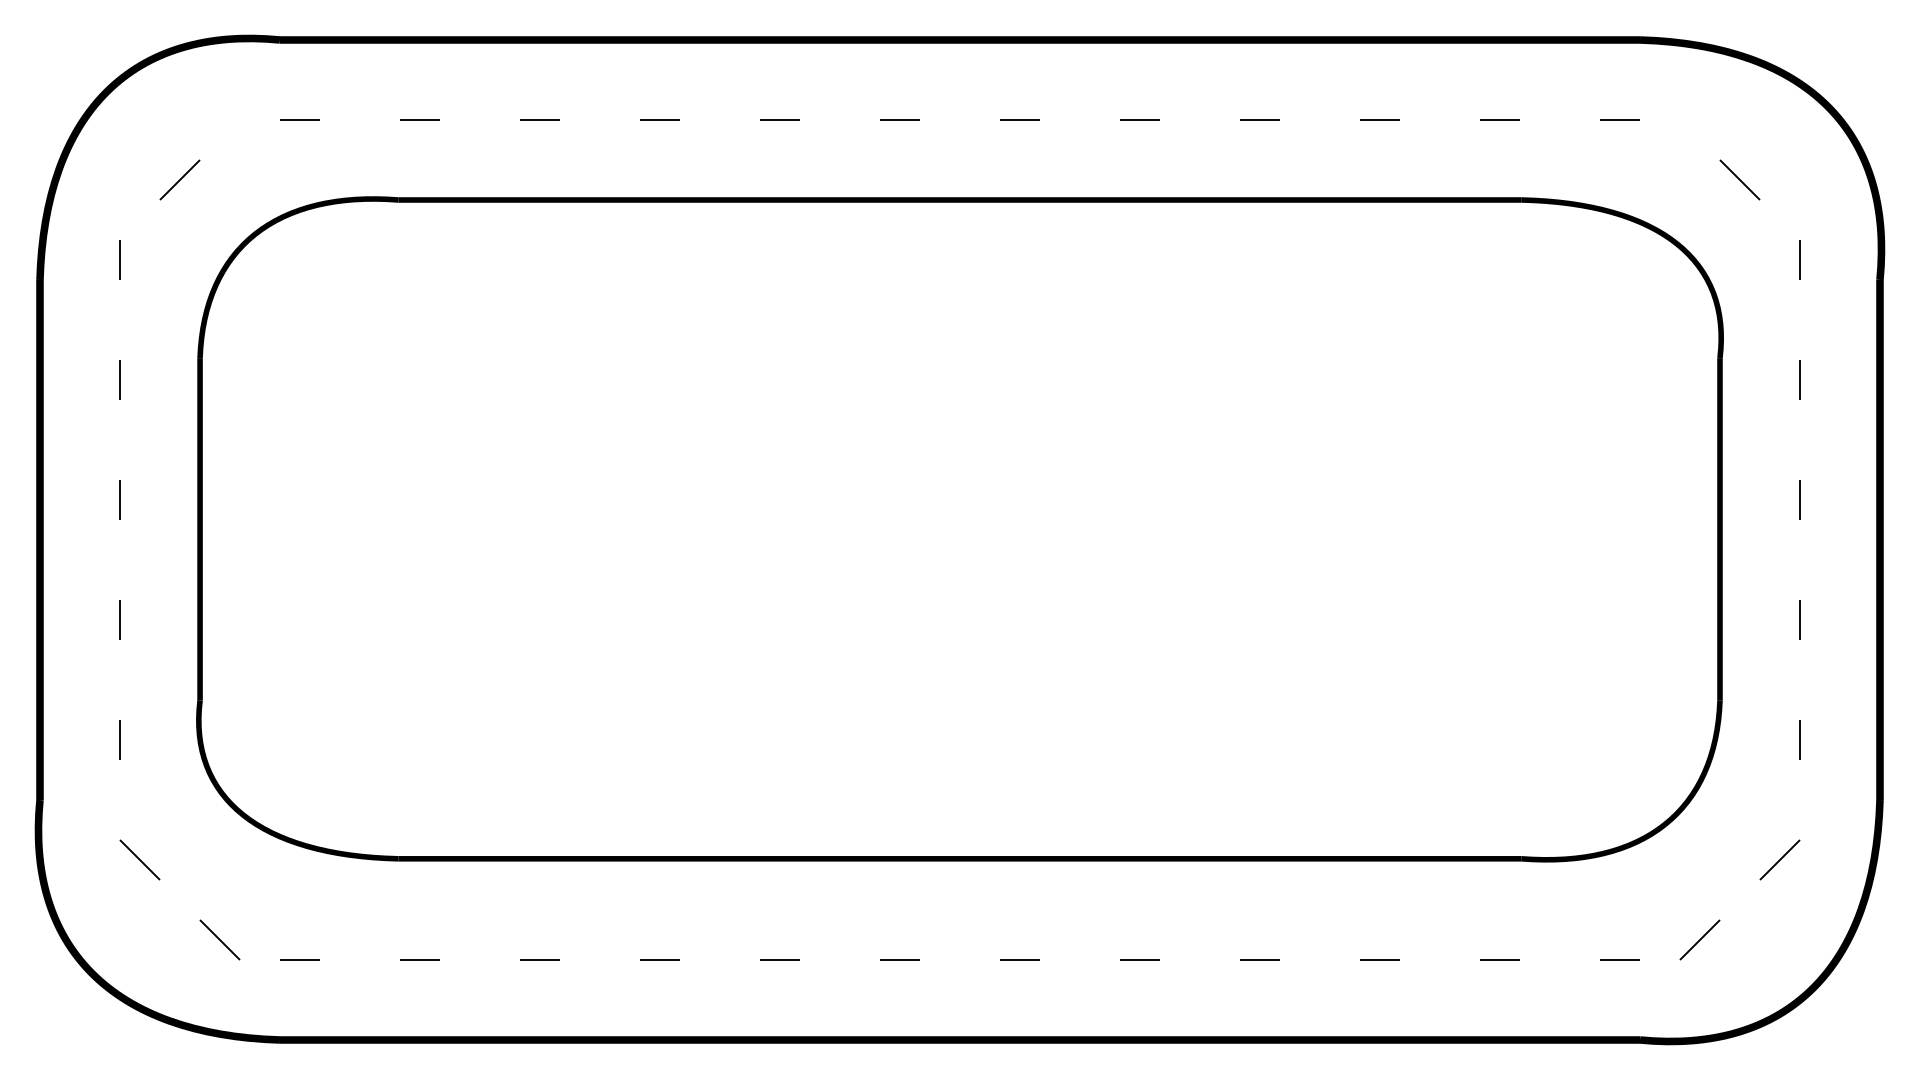
\includegraphics[width=.85\textwidth]{images/oval_track.png}
    \caption{AWS re:Invent 2018 track}
    \label{fig:track}
\end{figure}

Before we considered building the track, we drew it on the floor in our robotics laboratory using duct tape. This was possible due to the floor being solid black, just like the road on the track. This variant has several drawbacks compared to a properly built track. Built like this the track is stationary and can not be removed without destroying parts of it. During removal it might even happen that the adhesive will leave stains on the floor, which then again need to be removed. The alternative, interlocking foam pieces, are transportable and more durable, as they can be easily removed and rebuild as needed. Their major drawback is the costs. While using duct tape as markings on the floor is cheaper and faster, using foam puzzles will be more efficient in the long run.

\section{The Material}
Choosing the right material for the track proved to be straightforward. At first we thought of interlocking foam pieces. Foam pieces provide many advantages compared to other materials. They are lightweight and easy to transport. Durability and thickness are not as important, as the track is not meant to be stepped on and our car does not cause much wear and tear. Far more important is the ability of the pieces to stick together. The tiles must not under any circumstances break away from each other, this could cause serious damage to the track and vehicle. The only downside was the price. As seen in the table below, laying out the entire loop would cost around 300 €. Our second option was to use duct tape as markings on the black floor in our laboratory. While it is not nearly as durable as the foam tiles, this method is far cheaper. In the end the decision fell on using duct tape markings on the floor for our first test runs. Therefor white and yellow duct tape was bought at a nearby hardware store.

%\begin{table}
% \caption{Material price comparison}
%\label{tab:materials}
% \centering
% \setlength{\tabcolsep}{5mm}
% \def\arraystretch{1.25}
% \begin{tabular}{|r|r|c|c|}
% \hline
% \textbf{Material} & \textbf{Price} \\
% \hline\hline
% Black foam tiles & 299.85 € \\
% \hline
% Duct tape on floor & 59.85 € \\
% \hline
% \end{tabular}
% \end{table}
% ToDo: Rewrite section
\subsection{Track and Field Colour}
The material is not the only factor we need to consider when building the track. Since our model is trained in a simulation with a specific colour scheme, we went to recreate this colour set in order to achieve the best performance. The road is the easiest to paint, as its colour is solid black with orange markings in the middle. The green area which covers most of the track is far more difficult to recreate. This leads to two options:
%\begin{itemize}
%    \item Black foam tiles, either paint the background green or leave it black
%    \item Green foam tiles, where the road has to be drawn on
%\end{itemize}
%\end{comment}

\section{Building the track}
After the decision on the material was final,  the process of building the track began. For multiple reasons we were required to increase the size of our track, which lead to the track being 204" long and 162" wide. The width of the road was reduced to 22". This, combined with the uneven floor, made accurate measurements difficult. Therefor the track borders have an average derivation of 0.8". In contrary to our expectations the duct tape proved to be durable enough. Other than the tape on the floor representing the road markings, no other materials were used. This means there were no vertical borders around the track. This lead to multiple occasions where the vehicle went off track and ran into an obstacle before it could stop.

\subsection{Side borders}
Our first course did not have any railings or borders on the side which would have prevented the car from going off track too far. The main purpose of these borders would have been to keep the vehicle from driving into obstacles around the track. Although the car is supposed to stop should it recognise that it went off the track, it happens that due to its speed it is not able to slow down in time. The barriers on the track limits serve the purpose to stop the car without damaging it, should such a scenario as described above occur.

The secondary purpose of the barriers is to provide a solid colour background, preferably in contrast to the road. Similar side covers can be seen during official tournaments. Recognising that it drove outside of the track limits is simpler and more consistent.
%\include{abbildungen}
%\include{mathematik}
%\include{literatur}
%\include{drucken}
%\include{word}
\include{schluss}

%%%----------------------------------------------------------
%%%Anhang
\appendix
%\include{anhang_a}	% Technische Ergänzungen
%\include{anhang_b}	% Inhalt der CD-ROM/DVD
%\include{anhang_c}	% Chronologische Liste der Änderungen
%\include{anhang_d}	% Quelltext dieses Dokuments

%%%----------------------------------------------------------
%Ausgabe der automatischen Zusatzdaten: Glossar, Index, Literaturverzeichnis
\clearpage
\printglossaries

\clearpage
\chapter*{Index}
\addcontentsline{toc}{chapter}{Index}
\printindex[allgemein]

\printindex

\printindex[name]

\printindex[title]


%Literaturverzeichnis
\clearpage
\addcontentsline{toc}{chapter}{\bibname}

\printbibliography


%%%----------------------------------------------------------

%%%Messbox zur Druckkontrolle
%\include{messbox}

\end{document}
